\documentclass[a4paper, 12pt]{article}
\usepackage{amsmath}
\usepackage{amsfonts}
\usepackage{amssymb}
\usepackage{graphicx}
\usepackage{url}
\usepackage{subcaption}
\usepackage{times}
\usepackage{booktabs}
\usepackage{hyperref}
\usepackage{cleveref}
\usepackage{fancyhdr}
\usepackage{xcolor}
\usepackage{sidecap}
\usepackage[round]{natbib}
\bibliographystyle{abbrvnat}

\usepackage[
a4paper,
	%left=3cm,
	%right=3cm,
	%top=3cm,
	bottom=3.5cm,
 %headheight=0pt,
 %headsep=2pt
]{geometry}

% Header settings
\pagestyle{fancy}
\fancyhf{}
\chead{\textcolor{gray}{GNI Symposium \& Expo on Artificial Intelligence for the Built World\\
Technical University of Munich, September 10-12, 2024}}
\renewcommand{\headrulewidth}{0pt} % Remove the header line

%\pagenumbering{gobble}

\title{\large\textbf{A Comparative Study on the Urban Weather Generator:\\How Useful Is It for Urban Decision-Making?}}

\author{
\normalsize
Ze Yu Jiang$^{1}$, Sofia Mujica$^{2}$, Maryam Almaian$^{3}$, Patrick Kastner$^{3*}$\\
        \small $^{1}$School of Computer Science, Georgia Tech, Atlanta, USA \\
        \small $^{2}$George W. Woodruff School of Mechanical Engineering, Georgia Tech, Atlanta, USA \\
        \small $^{3}$School of Architecture, Georgia Tech, Atlanta, USA \\
        \small $^{*}$Corresponding author: \href{patrick.kastner@gatech.edu}{patrick.kastner@gatech.edu} \\
}
\date{}

\begin{document}

\maketitle
\thispagestyle{fancy} % Apply the header style to the first page

\vspace{-1.5cm}

\subsection*{Introduction}

Microclimates are localized regions in which the environmental conditions differ from those of the surrounding areas. 
As urban areas continue to develop and expand, sustainable urban planning becomes increasingly crucial to manage and mitigate global warming.
%The microclimate is influenced by various environmental factors, including wind velocity, relative humidity, and ambient temperature. 


Accurately determining and measuring these factors is essential for sustainable urban decision-making, as urban morphology influences these factors and can reduce heat islands in cities \citep{tehrani_predicting_2024}.
Previous research focuses on modeling building agglomerations, but most tools generally cannot simulate larger areas due to computational overhead \citep{singh_recent_2024}.
The Urban Weather Generator (UWG) is a tool that estimates hourly canopy air temperatures using environmental boundary conditions and cursory information on building geometries \citep{mao_urban_2021}.

Urban campuses, such as Georgia Tech University in Atlanta, Georgia, face campus growth and the impacts of added infrastructure; see \Cref{fig:campus-map}.
These universities require accessible tools, such as the UWG, to weigh the trade-offs of their campus expansion plans with the accompanying environmental impacts.
This study will evaluate whether the UWG could be a cost-effective alternative to its more expensive counterparts.

%\enlargethispage{1cm}


\subsection*{Methods}
The UWG operates on an EnergyPlus Weather (EPW) file representing the location of interest and the user's input on urban morphology and specific boundary conditions, including those on climate. 
Then it outputs an EPW file with predicted temperatures under given conditions \citep{nakano2015urban}.
Of the 54 input parameters, we isolated 14 (see \Cref{fig:radial-plot})  for which data could reasonably be obtained with reasonable time and effort.
A variance-based sensitivity analysis (SA) \citep{lo_piano_variance-based_2021} was performed to receive the first (individual importance), second (covariance), and total order (total effect) indices of the parameters, which will be used to rank-order the most influential parameters for the simulation; see \Cref{fig:sensitivity-indices}.
We used the root mean squared error between the canyon temperature (output) and the dry bulb temperature (input) from Jan. 1-10 as an objective function for the SA.

Running 100,000 samples for the sensitivity analysis produced the results shown in \Cref{fig:radial-plot}. 
The total order is prevalent for all 14 parameters as all were included for the campus simulation, despite most having nearly negligible first-order values. 
This study validates that the UWG produces an EPW with a mean absolute error and a mean square error of approximately 3.81 and 24.24 degrees, respectively, from the input file, proving that it is an efficient model for hourly urban canopy and air temperatures in urban microclimates.

\begin{figure}[htb]
    \centering
    \begin{minipage}[b]{0.48\textwidth}
        \centering
        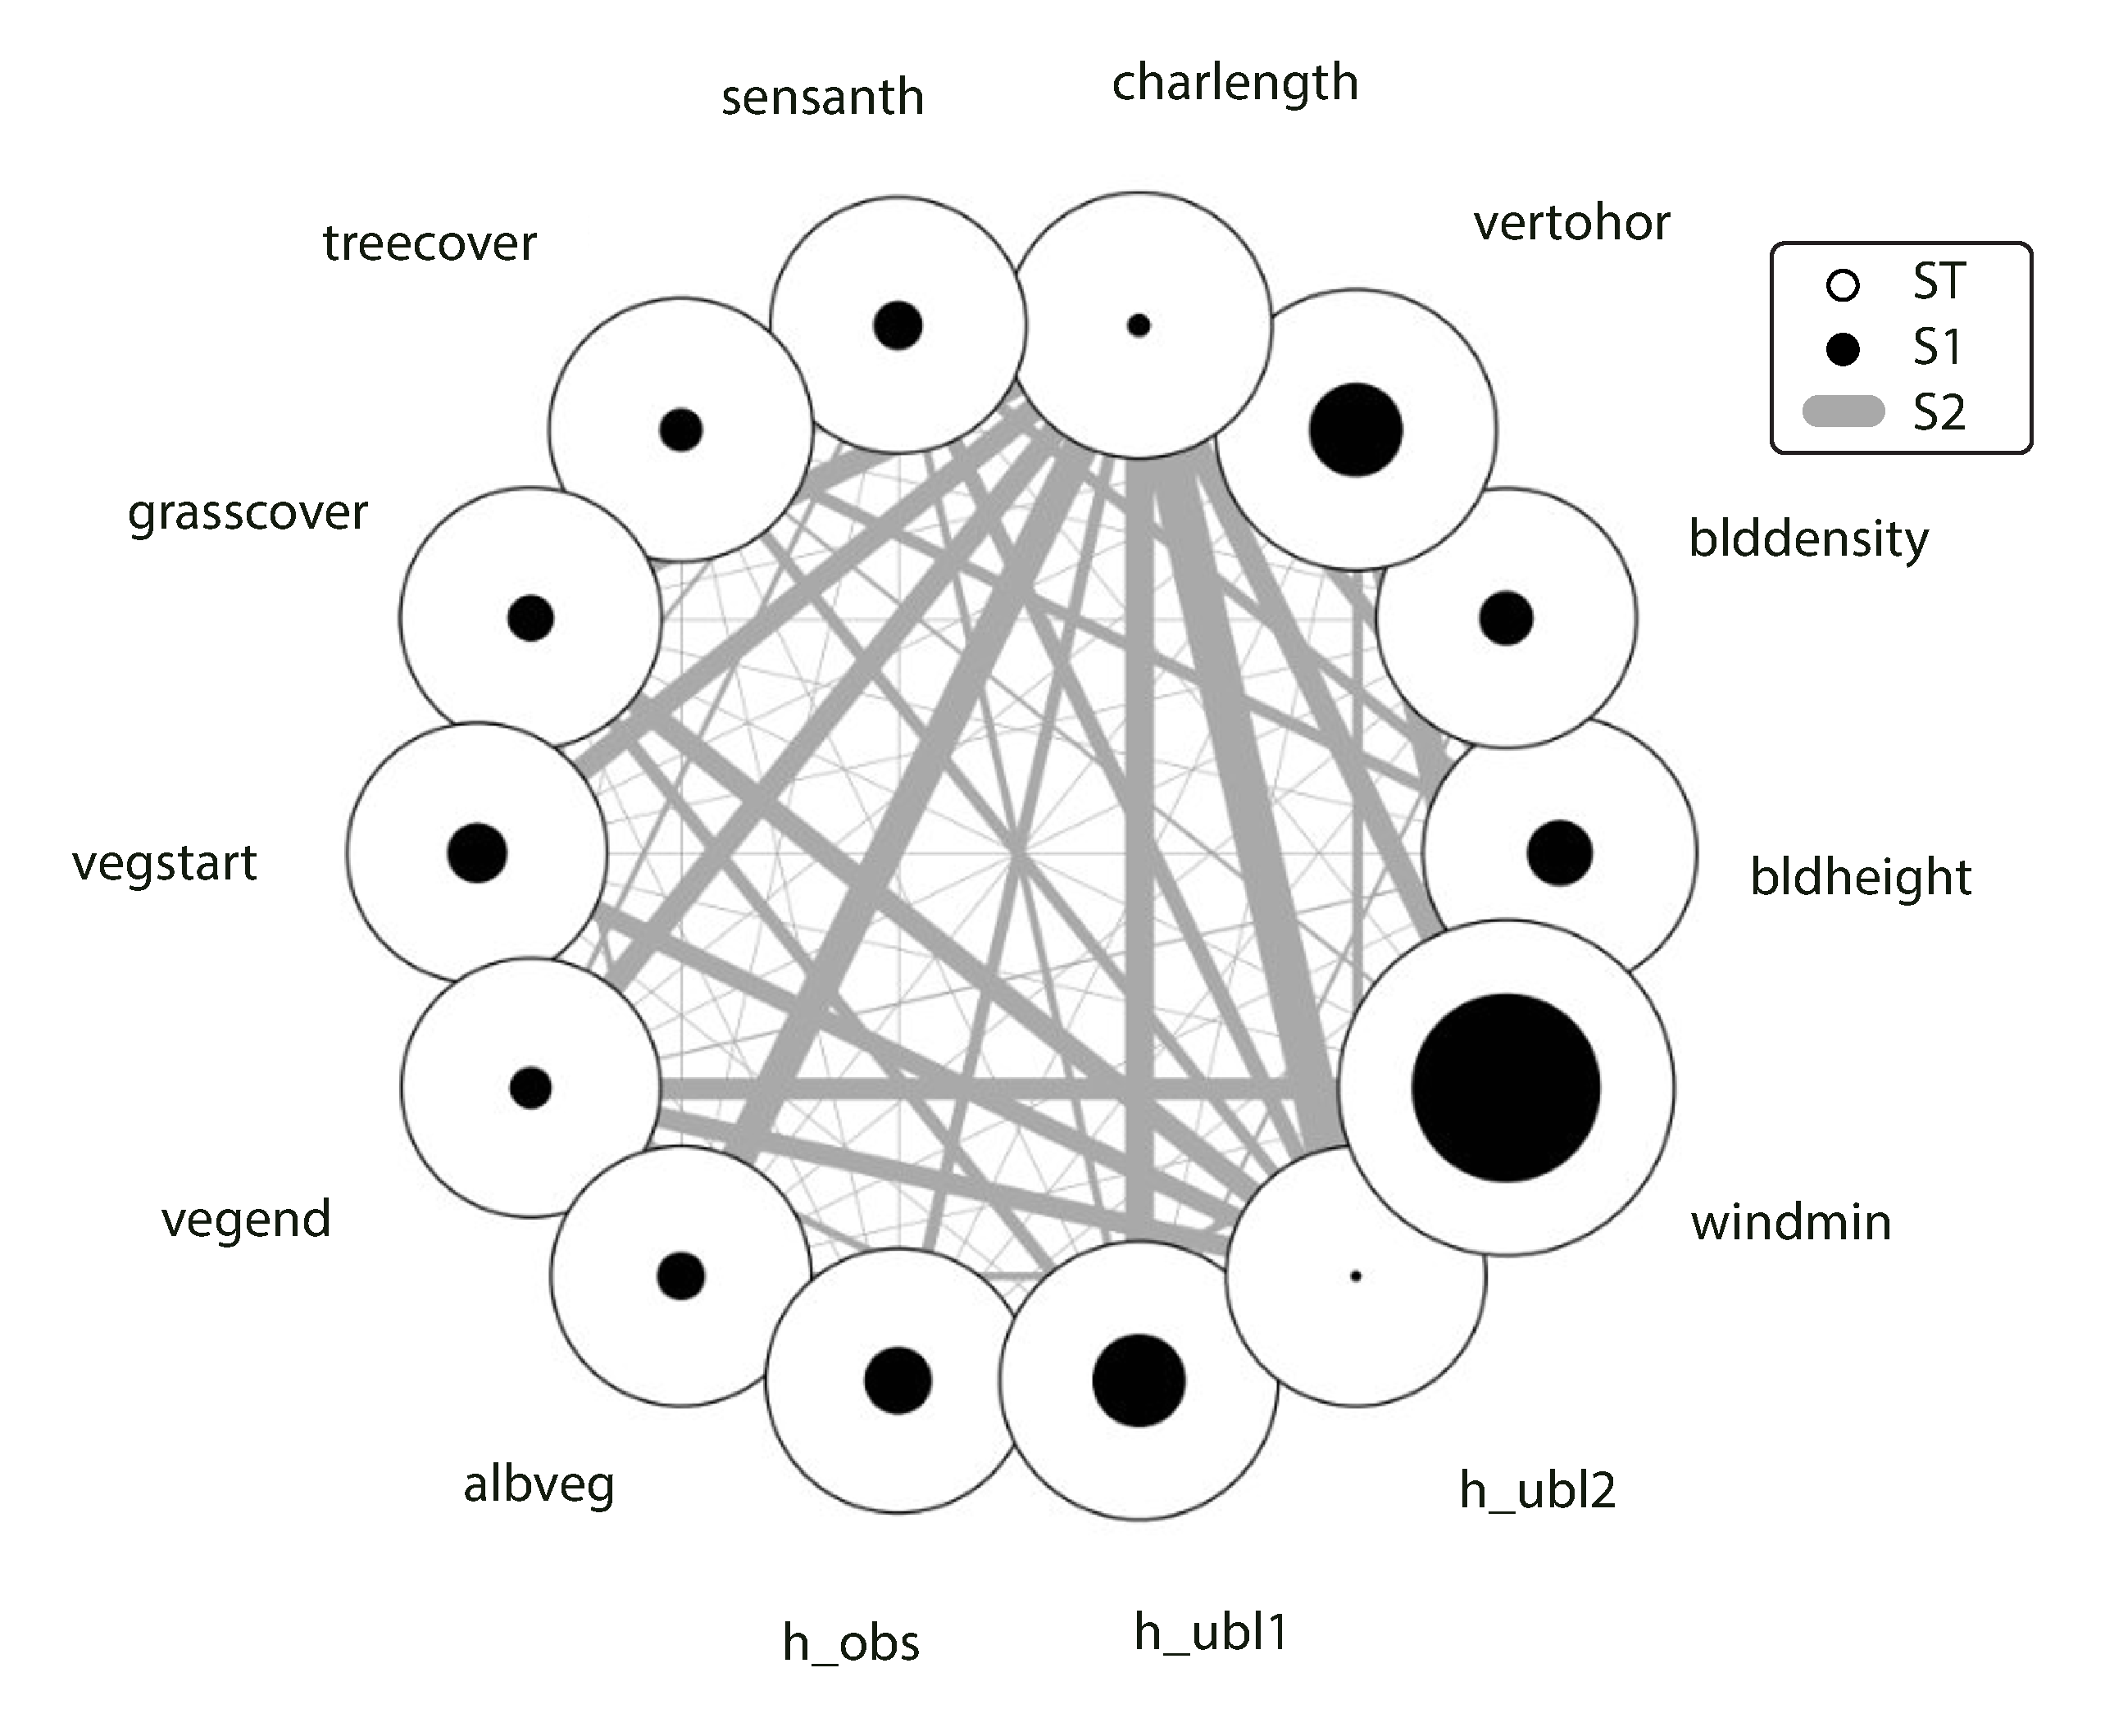
\includegraphics[width=\textwidth, trim = 0.5cm 0.5cm 0.5cm 0.5cm, clip = true]{Figures/UWG_Sensitivity.pdf}
        \caption{First, second, and total sensitivity indices of selected input parameters.}
        \label{fig:radial-plot}
    \end{minipage}
    \hfill
    \begin{minipage}[b]{0.48\textwidth}
        \centering
        \scriptsize
        \begin{tabular}{lrr}
        \toprule
        \textbf{Parameter} & \textbf{S1} [\%] & \textbf{ST} [\%] \\
        \midrule
        Wind Min Speed & 0.25 & 0.85 \\
        Vertical Horizontal Ratio & 0.05 & 0.59\\
        Urban Bound Layer (Day) & 0.05 & 0.57 \\
        Rural Avg Obst Height & 0.02 & 0.52  \\
        Veg Start Month & 0.01 & 0.50 \\
        Avg Bld Height & 0.01  & 0.56   \\
        Bld Density (BD) &  $<$0.01      & 0.50   \\
        Grass Cover (GC) &   $<$0.01    &  0.50   \\
        Albedo of Veg &  $<$0.01    &  0.50  \\
        Sensible Heat &  $<$0.01    &  0.48  \\
        Tree Cover (TC) &    $<$0.01     &  0.51  \\
        Veg End Month &  $<$0.01     & 0.50  \\
        Neighborhood Length &  $<$0.01  & 0.53  \\
        Urban Bound Layer (Night) &  $<$0.01  &  0.50   \\
        \bottomrule
        \end{tabular}
        \caption{Highest to lowest first-order sensitivity indices.}
        \label{fig:sensitivity-indices}
    \end{minipage}
\end{figure}

The team extracted data from the \textit{KGAATLAN216} weather station available on Wunderground to gather weather data local to the Georgia Tech campus.
There is a station located at Tech's Campus Recreation Center, shown in \Cref{fig:campus-map}.
This data provides us with the necessary campus weather information that meets the variable criteria of the UWG.
To post-process the data, we resampled the sub-hourly data to the closest hour, respecting the mean. 
%By element inspection on Wunderground, XPath is used to set the variable outputs into an array for 365 days to form a temporary EPW file.
The input variables are summarized in \Cref{tab:input_variables}.


\begin{table}[!ht]
\footnotesize
%\scriptsize
    \centering
    \caption{Input variables for the reference weather station and Science Square expansion.}
    \begin{tabular}{lll}
    \toprule
        \textbf{Variables} & \textbf{Reference} & \textbf{Science Square} \\ \midrule
        Grass cover & 47.2 \% & 55.4 \% \\ 
        Tree cover & 11.5 \% & 18.5 \% \\ 
        Building density & 45.4 \% & 6.6 \% \\ \bottomrule
    \end{tabular}
    \label{tab:input_variables}
\end{table}
%\vspace{-0.5cm}



\begin{figure}[tbhp]
    \centering
    \begin{minipage}[b]{0.49\textwidth}
        \centering
        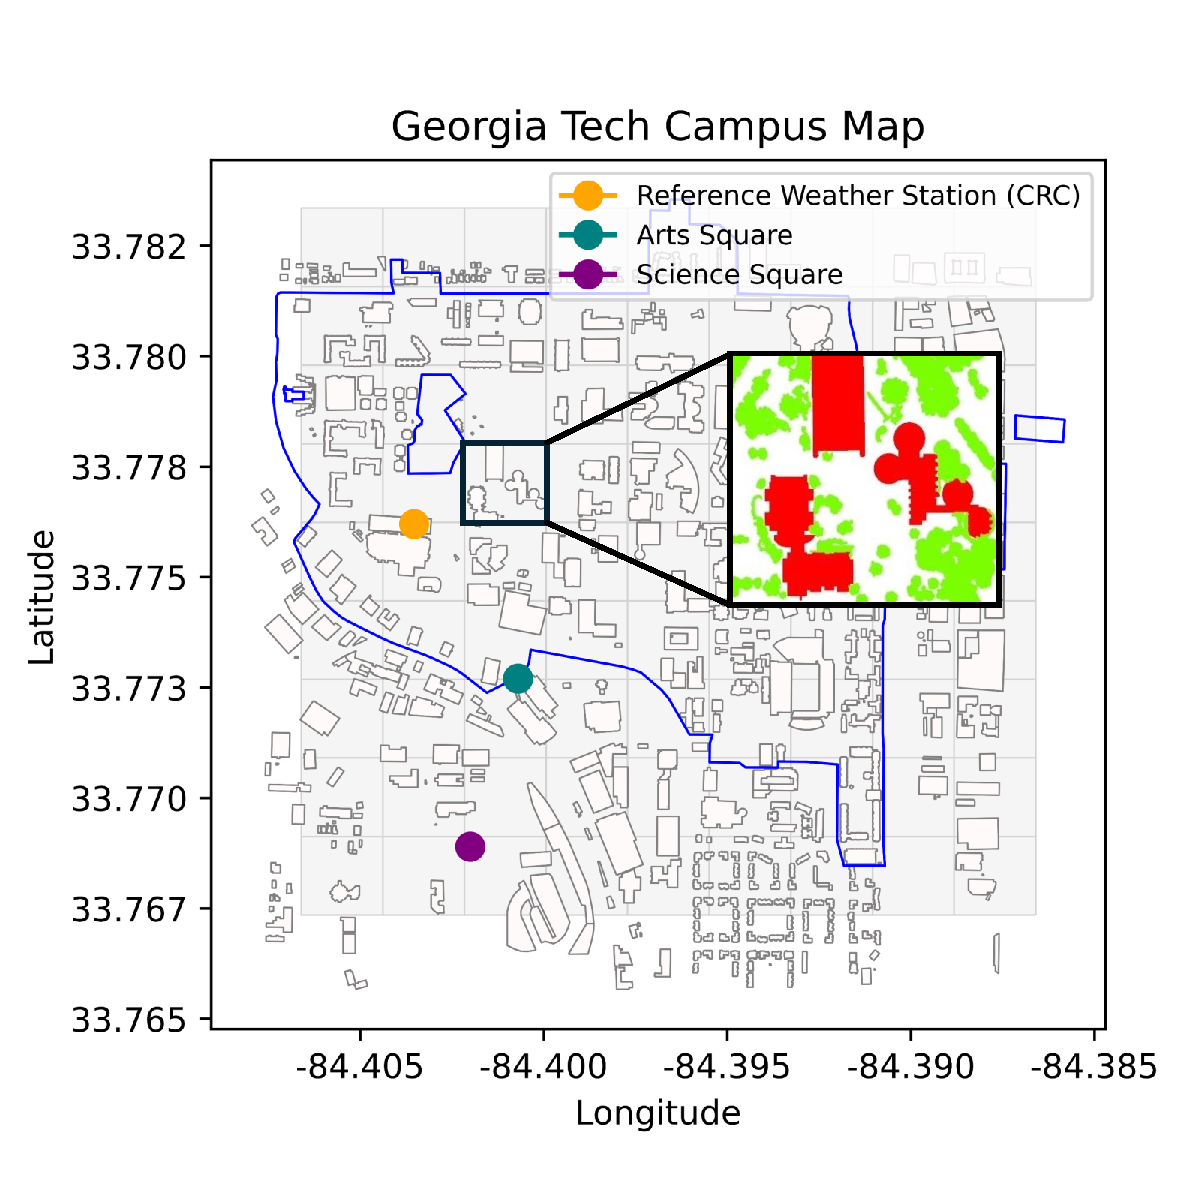
\includegraphics[width=\textwidth, trim = 0.45cm 0.80cm 0.40cm 2.7cm, clip = true]{Figures/georgia_tech_map_with_tiles.pdf}
        \caption{Campus with CRC weather station, campus expansion sites \textit{Science Square} and \textit{Arts Square}, and callout illustrating exemplary building and vegetation density.}
        \label{fig:campus-map}
    \end{minipage}
    \hfill
    \begin{minipage}[b]{0.49\textwidth}
        \centering
        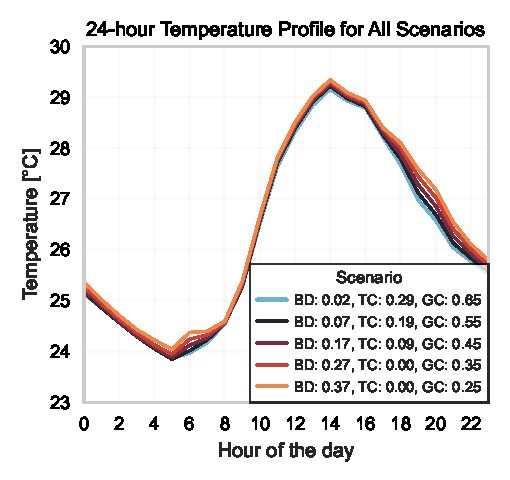
\includegraphics[width=1\textwidth, trim = 0.1cm 0.1cm 0.1cm 0.68cm, clip = true]{Figures/Diurnal_Hottest_Month_July.pdf}
        \caption{Diurnal UWG output for July for proposed \textit{Science Square}, denoting current proposal in black. Other scenarios denote varying building density (BD), tree cover (TC), and grass cover (GC).}
        \label{fig:comparing-epw}
    \end{minipage}
\end{figure}

\subsection*{Results}

\Cref{fig:comparing-epw} shows the dry bulb temperature on April 5, 2023, for the reference condition and the Science Square campus extension. 
The results show a difference of 0.1-0.3°C for both locations throughout the day, with the maximum occurring in the early afternoon.
The temperatures during the night are identical.


\enlargethispage{1cm}

\subsection*{Discussion \& Conclusion} 

A major limitation of this analysis is the assumed homogeneity for environmental parameters, such as wind velocity, which typically exhibit spatial and diurnal fluctuations. UWG in its current state does not support dynamic inputs for these.

For the sensitivity analysis, we were required to manually limit the input ranges of grass cover, tree cover, and building density to ensure that their sum does not exceed 1 for the Sobol sensitivity analysis, ignoring any overlap.

Further work will include resolving issues from the Mercator tiling approach to evenly divide campus data for more detailed output. 
This approach will allow for partitioning of the campus into subsets of bounded regions. 
Using the edge coordinates, we can retrieve the parameter values of the subregions and simulate each. 
This would provide increased accuracy in simulating the overall dry bulb temperature in the regions of interest.


\enlargethispage{1cm}


\footnotesize
\scriptsize
%\tiny
\bibliography{bib.bib}

\end{document}
